\chapter{مدیریت و وضعیت سرور}
برای آنکه یک ابزار را نصب کنید یا باید از مخازن نصب شود یا اینکه از طرق مختلفی اقدام به نصب آن کنید. برخی موارد ابزارها در اینترنت و پایگاه اینترنتی گیت‌هاب قرار دارند. ابزار اطلاعات سرور، ابزاری است که در گیت‌هاب قرار دارد و برای نمایش اطلاعات سرور به کار می‌رود. برای اجرای آن ابتدا باید آن را بارگیری کرد. در این صورت شما نیاز به نصب ابزار گیت برای بارگیری ابزار بالا دارید که آن را با دستور زیر نصب خواهید کرد. اگر ابزار بالا نصب شود باید برنامه از گیت‌هاب بارگیری شود و سپس به پوشه مورد نظر می ‌رویم تا ببینیم چه چیزی در آن وجود دارد.

بعد از آنکه کد بالا بارگیری شد، و به پوشه مورد استفاده در آپاچی منتقل شد. سپس با استفاده از روش بالا، آدرس آن را در جدول میانبرها وارد می‌کنیم تا بتوانیم آن را به پیشخوان اضافه کنیم. این کد در این پیوند به گیت‌هاب نیز قابل دریافت است. برای دریافت کدها دستورات زیر را اجرا کنید.
\newline

\begin{latin}  
    \lstinputlisting[numbers=right,language=SH, framexleftmargin=5mm, frame=shadowbox,rulesepcolor=\color{Black}]{Code/server-status.sh}
\end{latin}

همانطور که در دستورات بالا و در آخرین دستور مشخص است چند فایل توسط این دستور دریافت شده است. اگر با استفاده از دستور «Cat» مقادیر فایل «README» را مشاهده کنید، خواهید دید که برای استفاده از کد بالا باید چه کارهایی را انجام دهید. اولین قدم را که ساخت یک بانک اطلاعاتی برای این  صفحه است را با دستور مشابه دستورات ذکر شده انجام داده و بانک اطلاعاتی مربوط به ابزار به همراه نام کاربری مناسب را نیز ایجاد می‌کنیم.همانند کاری که برای بانک اطلاعاتی سندباکس و پیشخوان انجام دادیم.  با این حال اگر نمی‌خواهید بانک و کاربر جدید را ایجاد کنید، در این سرور ما یک کاربر سندباکس داریم که برای این‌کار می‌توان از آن استفاده کرد. اما بهتر است یک نام کاربری به همراه یک بانک اطلاعاتی جداگانه ایجاد کنید تا برای این برنامه استفاده شود.\newline

\begin{latin}  
    \lstinputlisting[numbers=right,language=SQL, framexleftmargin=5mm, frame=shadowbox,rulesepcolor=\color{Green}]{Code/server-status.sql}
\end{latin}

سپس به یک شاخه قبل برگشته و با دستور زیر شاخه بارگیری شده را به شاخه مورد استفاده و به اشتراک گذاشته شده بین سرور و اوبونتو منتقل کنید.
\newline

\begin{latin}  
    \lstinputlisting[numbers=right,language=SH, framexleftmargin=5mm, frame=shadowbox,rulesepcolor=\color{Black}]{Code/server-status2.sh}
\end{latin}

بعد از آن به پوشه «sql» واقع در پوشه «server-status» را وارد، مای‌اس‌کیوال کنید. برای این‌کار از دستور زیر را در خط رمان اوبونتو سرور وارد کنید.
\newline

\begin{latin}  
    \lstinputlisting[numbers=right,language=SH, framexleftmargin=5mm, frame=shadowbox,rulesepcolor=\color{Black}]{Code/server-status3.sh}
\end{latin}

اگر دستورات بالا با موفقیت اجرا شود، فایل 
\path{«/includes/config.php»}
 را ویرایش کرده و تنظیمات بانک اطلاعاتی را به مقادیر دلخواه تغییر می‌دهیم. به عنوان نمونه برای مثال فایل بالا بعد از تغییر به صورت زیر خواهد بود. فایل بالا را می‌توانید توسط سیستم میزبان و در داخل ویرایشگر پیشرفته‌تر مانند اتم «Atom» هم ویرایش کنید.
\newline

\begin{latin}  
    \lstinputlisting[numbers=right,language=PHP, framexleftmargin=5mm, frame=shadowbox,rulesepcolor=\color{Blue}]{Code/server-status-config.php}
\end{latin}

تصویری از ویرایشگر اتم، در زمان ویرایش فایل مذکور نیز در زیر آمده است. بعد از این تمامی فایل‌ها را با استفاده از یک ویرایشگر که در سیستم میزبان نصب است ویرایش خواهیم کرد. سپس می‌توانید دیگر تنظیمات و موارد را نیز بر اساس راهنمای ابزار بالا انجام دهید. همانطور که مشاهده کردید، نصب یک نرم‌افزار و یا یک صفحه آماده از طریق گیت‌هاب کار بسیار ساده‌ای است. در این حالت شما می‌توانید اکثر ابزارهای مورد نیاز خود را از طریق گیت‌هاب دریافت کنید و با استفاده از راهنمای موجود در فایل مرا بخوان «README» آنان را نصب و تنظیم کنید. )(\ref{SERVER-STATUS-ATOM-EDITOR})
\begin{figure}
    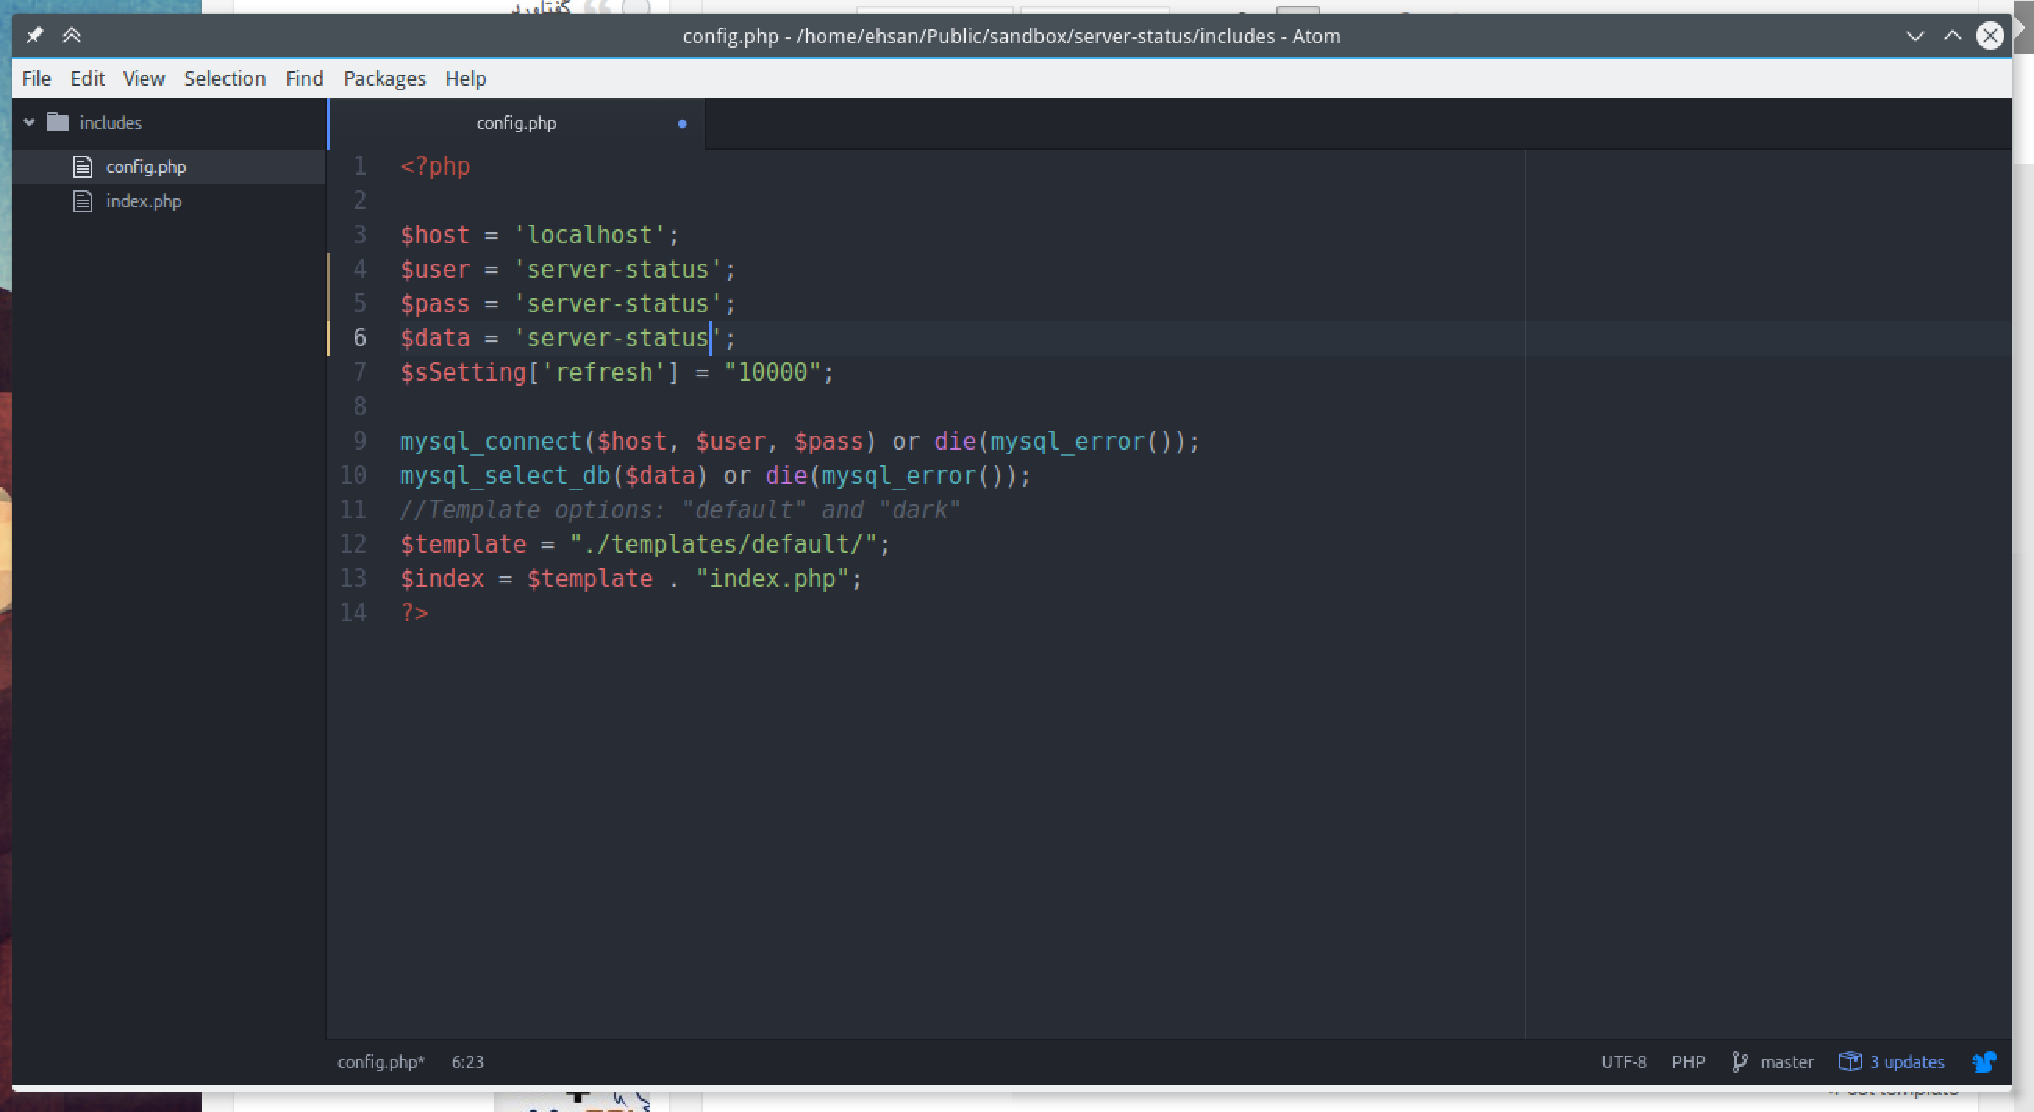
\includegraphics[width=.9\textwidth ,height=.60\textwidth]{Pic/SERVER-STATUS-ATOM-EDITOR}
    \caption{ ویرایش تنظیمات نرمافزار وضعیت سرور در اتم
        \lr{(Atom)}   
    }
    \label{SERVER-STATUS-ATOM-EDITOR}
\end{figure}

\section{مدیریت سرور با ابزار گرافیکی}
استفاده از دستورات خط فرمان برای مدیریت یک سرور معمولا کاربردی هستند، با این حال به خاطر سپردن اکثر دستورات خط فرمانی و انجام تغییرات در یک سرور نیازمند تنظیماتی است که اگر از تنظیمات گرافیکی استفاده شود تا حدودی کارها برای شما ساده‌تر خواهد بود. یکی از ابزارهای گرافیکی تنظیم یک سرور آجنتی «Ajenti» نام دارد. این ابزار ابزاری متن‌باز / آزاد است که برای کاربرد مورد نظر ما در یک سرور محلی به صورت سندباکس بسیار مناسب خواهد بود. این نرم‌افزار در مخازن اوبونتو در دسترس نیست و باید برای نصب آن از دستورات زیر استفاده کنید.
\newline

\begin{latin}  
    \lstinputlisting[numbers=right,language=SH, framexleftmargin=5mm, frame=shadowbox,rulesepcolor=\color{Black}]{Code/anjeti.sh}
\end{latin}
دستور بالا با دانلود اسکریپت نصاب و اجرای آن، باعث نصب ابزار بالا می‌شود. بعد از نصب گذرواژه و نام کاربری نیز  در پیغام نمایش داده شده مشخص شده است.
\newline

\begin{latin}  
    \lstinputlisting[numbers=right,language=Tex, framexleftmargin=5mm, frame=shadowbox,rulesepcolor=\color{Black}]{Code/anjeti.txt}
\end{latin}

بعد از آن باید خدمت بالا را راه‌اندازی مجدد کنید، برای راه‌اندازی مجدد خدمت بالا باید دستور زیر را در خط فرمان اجرا کنید.
\newline

\begin{latin}  
    \lstinputlisting[numbers=right,language=SH, framexleftmargin=5mm, frame=shadowbox,rulesepcolor=\color{Black}]{Code/anjeti-restart.sh}
\end{latin}

خدمت بالا نیز نیاز به درگاه خاصی برای اجرا دارد. این درگاه فقط در در سندباکس مجاز است و همانند درگاه‌های مورد استفاده دیگر، آن را انتقال نداده‌ایم.  حال برای تنطیم مجدد موارد انتقال درگاه در نرم‌افزار اوراکل ویرچوال‌باکس، وارد تنظیمات انتقال درگاه در اوراکل ویرچوال‌باکس شده و مقادیر جدید را برای انتقال درگاه در این ابزار وارد کنید، آموزش نحوه افزودن یک درگاه برای انتقال را در قسمت اول آموزش داده‌ایم. در این مورد می‌خواهیم درگاه \path{8000} را مجددا به همان درگاه \path{8000} انتقال دهیم. با وجود این اگر درگاه \path{8000} در سیستم شما استفاده می‌شود، باید از درگاه دیگری استفاده کنید.  بعد از انتقال درگاه بالا، وارد پی‌اچ‌پی مای‌ادمین شوید و آدرس دسترسی به برنامه را نیز به پیوندهای موجود در پیشخوان بیفزایید. آدرس دسترسی به این ابزار به صورت زیر خواهد بود. بعد از وارد شدن به آدرس زیر باید نام‌کاربری و رمز‌عبور نوشته شده در پیغام نصب را وارد کنید. این پیغام به صورت کادری کوچک نمایش داده شده است که گزینه‌ای برای ذخیره مقادیر وارد شده برای مواقع بعدی و یا حتی ورود برای همیشه در آن وجود ندارد. به دلیل آنکه این گذرواژه امنیت پایینی دارد، پیشنهاد می‌شود سریعا بعد از ورود به آن، گذرواژه جدیدی را انتخاب کنید.

\begin{latin}
\url{https://sandbox.dev:8000/}
\end{latin}

بعد از نوشتن آدرس بالا با صفحه‌ای مطابق شکل زیر مواجه خواهید شد. اگر پیغام هشداری برای عدم اعتبار اچ‌تی‌تی‌پی‌اس، مشاهده کردید آن را نادیده گرفته و وارد صفحه اصلی شوید. این هشدار برای ناشناس بودن هویت این پایگاه است که به دلیل استفاده محلی و در سندباکس نادیده گرفتن آن مشکل خاصی را به دنبال نخواهد داشت. \ref{SERVER-MANAGER-ANJETI1}

\begin{figure}
    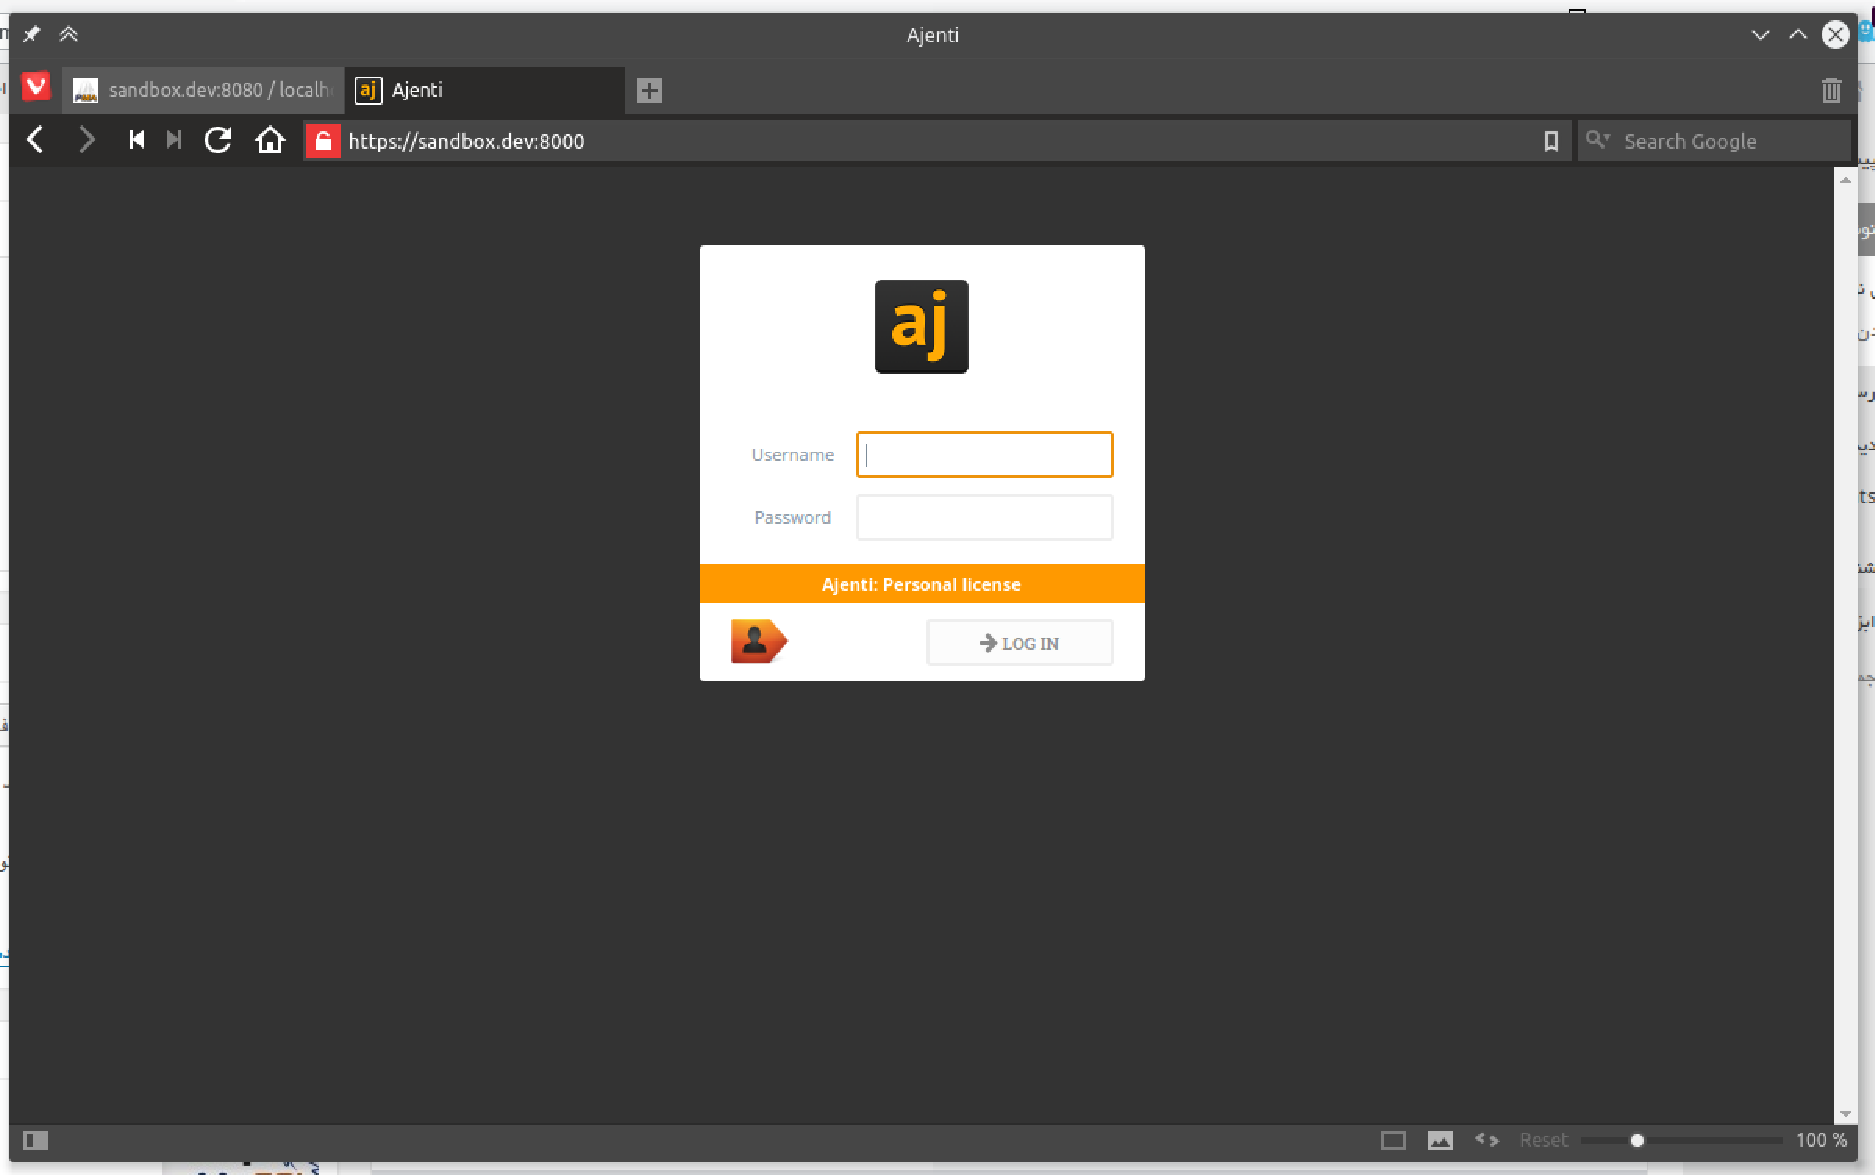
\includegraphics[width=.9\textwidth ,height=.60\textwidth]{Pic/ANJETI1}
    \caption{ محیط ورود به حساب کاربری
        \lr{(Anjeti)}   
    }
    \label{SERVER-MANAGER-ANJETI1}
\end{figure}

بعد از وارد کردن نام‌کاربری و گذرواژه گفته شده در بالا یعنی «root» و «admin»، به بخش اصلی نرم‌افزار وارد خواهید شد. با وجود اینکه این سرور در یک سندباکس است، بهتر است گذرواژه بهتری را بر گزینید. برای این کار از قسمت سمت چپ بر روی پیوند تنظیم «Configure» کلیک کرده  و در پایین صفحه در قسمت گذرواژه، گذرواژه بهتری را وارد کرده و تنظیمات را ذخیره کنید. در زیر نمایی از صفحه اول این ابزار را مشاهده می‌کنید که شامل اطلاعاتی از سرور، مانند مقدار حافظه مصرف شده و اطلاعات زمان اجرا یا حتی پردازنده نیز هستید.
\ref{SERVER-MANAGER-ANJETI2}
\begin{figure}
    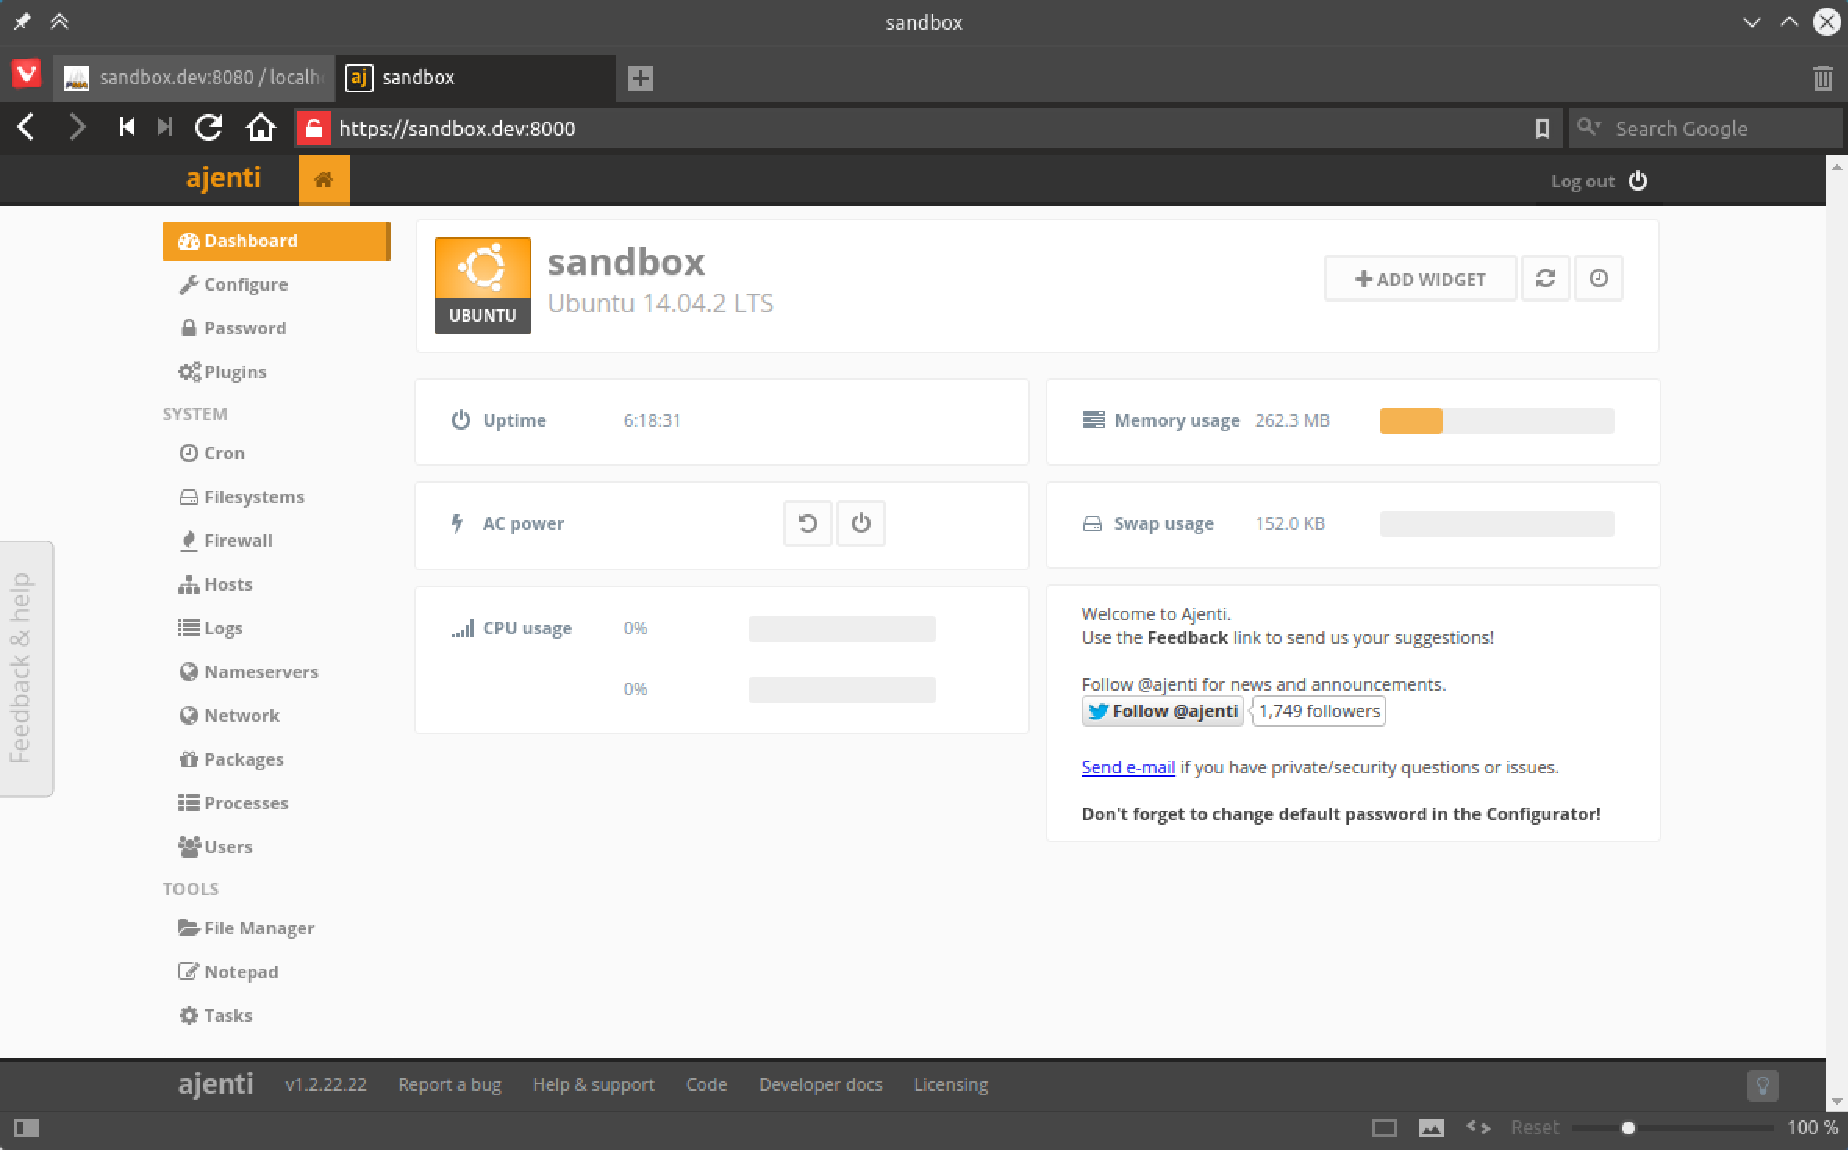
\includegraphics[width=.9\textwidth ,height=.60\textwidth]{Pic/ANJETI2}
    \caption{ محیط ورود به حساب کاربری
        \lr{(Anjeti)}   
    }
    \label{SERVER-MANAGER-ANJETI2}
\end{figure}

در این چند فصل به معرفی و آموزش ابزارهای گرافیکی و تحت وب برای مدیریت و بررسی وضعیت سرور پرداختیم. یکی از این ابزارها پی‌اچ‌پی مای‌ادمین نام داشت که برای مدیریت بانک‌های اطلاعاتی مای‌اس‌کیوال کاربرد داشته و قادر است اکثر کارهای معمول را انجام دهد. با این حال ابزار بالا معمولا در محیط‌هایی که به امنیت بالایی نیاز دارند، نصب نمی‌شود. ابزار گرافیکی مدیریت کارساز وب و سرور آجنتی نیز با وجود تنظیمات بسیار خوبی که به همراه دارد، برای سرورهای تجاری مناسب نیست اما استفاده از آن در یک سندباکس مشکل خاصی را به وجود نخواهد آورد.

بعد از انجام مراحل گفته شده در بالا هنوز هم برخی نکات قابل مطرح شدن هستند که این موارد را به فصل هفتم و هشتم یعنی یک یا دو قسمت بعد واگذار خواهم کرد. می‌توان گفت که فصلهای بعدی، قسمتی برای معرفی چند ابزار برای رفع ایراد کدهای پی‌اچ‌پی و همچنین ابزارهایی برای مدیریت یک پروژه خواهد بود. در این آموزش خواهید توانست تا گیت را تنظیم و از آن استفاده کنید. در فصل بعدی بر روی پروژه‌ها، مدیریت و رفع اشکال از خطاهای احتمالی متمرکز خواهیم بود.